% Source PDF page 191 (printed p. 177)
寻找 $x$ 的无偏估计的问题，可以表述为向量优化问题
\begin{equation}
\begin{array}{ll}\text{最小化（关于 }\mathbf S_+^n\text{）}&FF^\T\\\text{约束为}&FA=I,\end{array}\tag{4.58}
\end{equation}
变量为 $F\in\R^{n\times m}$。目标 $FF^\T$ 关于 $\mathbf S_+^n$ 凸，所以（4.58）是凸向量优化问题。一个简单证明是：对任意固定 $v$，$v^\T FF^\T v=\norm{F^\T v}_2^2$ 是 $F$ 的凸函数。

一个著名结果指出，（4.58）有最优解，即最小二乘估计或伪逆
\[
F^\star=A^\dagger=(A^\T A)^{-1}A^\T.
\]
对任意满足 $FA=I$ 的 $F$，有 $FF^\T\succeq F^\star F^{\star\T}$。矩阵
\[
F^\star F^{\star\T}=A^\dagger A^{\dagger\T}=(A^\T A)^{-1}
\]
是问题（4.58）的最优值。
\end{origexample}

\subsection{Pareto最优点与最优值}
现在考虑可达目标值集没有最小元的情形，这也是大多数有意义的向量优化问题的情况；此时问题没有最优点或最优值。可达值集的极小元在这些情形中起重要作用。若 $f_0(x)$ 是可达值集 $\mathcal O$ 的极小元，就称可行点 $x$ 为Pareto最优点，或有效点。此时称 $f_0(x)$ 为向量优化问题（4.56）的Pareto最优值。因此，$x$ 为Pareto最优点，意味着它可行，且对任意可行点 $y$，$f_0(y)\preceq_K f_0(x)$ 蕴含 $f_0(y)=f_0(x)$。换言之，任意优于或等于 $x$ 的可行点 $y$，即满足 $f_0(y)\preceq_K f_0(x)$ 的点，其目标值必与 $x$ 完全相同。

点 $x$ 为Pareto最优点，当且仅当它可行且
\begin{equation}
(f_0(x)-K)\cap\mathcal O=\{f_0(x)\}\tag{4.59}
\end{equation}
（见§2.4.2）。集合 $f_0(x)-K$ 可解释为优于或等于 $f_0(x)$ 的值组成的集合，因此（4.59）表示：优于或等于 $f_0(x)$ 的可达值只有 $f_0(x)$ 本身。图4.8说明了这一点。

向量优化问题可以有多个Pareto最优值和最优点。Pareto最优值的集合记为 $\mathcal P$，满足
\[
\mathcal P\subseteq\mathcal O\cap\operatorname{bd}\mathcal O,
\]
即每个Pareto最优值都是位于可达目标值集边界上的可达目标值，见习题4.52。

% Source PDF page 192 (printed p. 178)
\begin{figure}[htbp]
\centering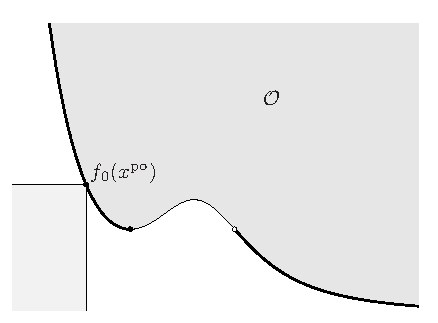
\includegraphics[width=.60\textwidth]{figures/ch04-08.pdf}
\caption*{图4.8\quad 向量优化的可达值集 $\mathcal O$ 为阴影部分，目标值位于 $\R^2$，锥为 $K=\R_+^2$。问题没有最优点或最优值，但有一组Pareto最优点，对应的值以 $\mathcal O$ 左下边界的粗曲线表示。标出的 $f_0(x^{\mathrm{po}})$ 是Pareto最优值，$x^{\mathrm{po}}$ 是Pareto最优点。浅阴影区域为 $f_0(x^{\mathrm{po}})-K$，即与优于或等于 $f_0(x^{\mathrm{po}})$ 的目标值对应的全部 $z\in\R^2$。}
\end{figure}

\subsection{标量化}
标量化是寻找向量优化问题的Pareto最优点或最优点的一种标准技巧，基于§2.6.3通过对偶广义不等式对最小元和极小元的刻画。任取 $\lambda\succ_{K^*}0$，即一个在对偶广义不等式下为正的向量。考虑标量优化问题
\begin{equation}
\begin{array}{ll}\text{最小化}&\lambda^\T f_0(x)\\\text{约束为}&f_i(x)\le0,\quad i=1,\ldots,m,\\&h_i(x)=0,\quad i=1,\ldots,p,\end{array}\tag{4.60}
\end{equation}
设 $x$ 为其最优点，则 $x$ 是向量优化问题（4.56）的Pareto最优点。这可由§2.6.3的极小元的对偶不等式刻画得到，也容易直接证明。若 $x$ 不是Pareto最优点，则存在可行 $y$ 满足 $f_0(y)\preceq_K f_0(x)$，且 $f_0(x)\ne f_0(y)$。由于 $f_0(x)-f_0(y)\succeq_K0$ 且非零，有 $\lambda^\T(f_0(x)-f_0(y))>0$，即 $\lambda^\T f_0(x)>\lambda^\T f_0(y)$，与 $x$ 为标量问题（4.60）的最优点矛盾。

借助标量化，可以通过求解普通标量优化问题（4.60），寻找任意向量优化问题的Pareto最优点。向量 $\lambda$ 有时称为权重向量，必须满足 $\lambda\succ_{K^*}0$。权重向量是自由参数；改变它，可能得到向量优化问题（4.56）的不同Pareto最优解，见图4.9。图中还给出一个Pareto最优点：对于任何权重 $\lambda\succ_{K^*}0$，它都不能由标量化得到。

% Source PDF page 193 (printed p. 179)
\begin{figure}[htbp]
\centering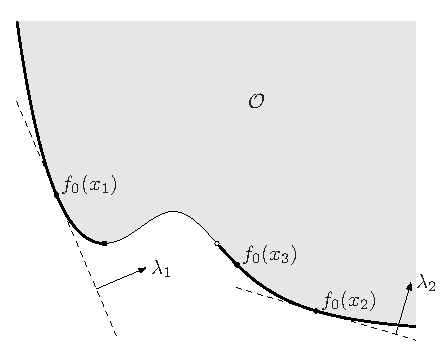
\includegraphics[width=.60\textwidth]{figures/ch04-09.pdf}
\caption*{图4.9\quad 标量化。向量优化问题的可达值集为 $\mathcal O$，锥为 $K=\R_+^2$。图中标出三个Pareto最优值 $f_0(x_1),f_0(x_2),f_0(x_3)$。前两个值可由标量化得到：$f_0(x_1)$ 在全部 $u\in\mathcal O$ 中最小化 $\lambda_1^\T u$，$f_0(x_2)$ 最小化 $\lambda_2^\T u$，其中 $\lambda_1,\lambda_2\succ0$。$f_0(x_3)$ 虽为Pareto最优值，却不能通过标量化得到。}
\end{figure}
标量化也有几何解释。点 $x$ 为标量化问题最优点，即在可行集上最小化 $\lambda^\T f_0$，当且仅当对所有可行 $y$，有 $\lambda^\T(f_0(y)-f_0(x))\ge0$。这等价于说，$\{u\mid-\lambda^\T(u-f_0(x))=0\}$ 在点 $f_0(x)$ 处是可达目标值集 $\mathcal O$ 的支撑超平面；特别地，
\begin{equation}
\{u\mid\lambda^\T(u-f_0(x))<0\}\cap\mathcal O=\varnothing.\tag{4.61}
\end{equation}
见图4.9。因此，求得标量化问题的最优点时，不仅得到原向量优化问题的一个Pareto最优点，还得到 $\R^q$ 中由（4.61）给出的整个半空间，其中目标值均不可达。

\subsubsection*{凸向量优化问题的标量化}
现在假设向量优化问题（4.56）凸，则标量化问题（4.60）也凸，因为由§3.6，$\lambda^\T f_0$ 是标量值凸函数。这意味着，可以通过求解凸标量优化问题，寻找凸向量优化问题的Pareto最优点。每选一个 $\lambda\succ_{K^*}0$，就得到一个通常不同的Pareto最优点。

对凸向量优化问题，有一个部分逆命题：每个Pareto最优点 $x^{\mathrm{po}}$ 都对应某个非零 $\lambda\succeq_{K^*}0$，使 $x^{\mathrm{po}}$ 是标量化问题（4.60）的解。粗略地说，对凸问题，让权重向量 $\lambda$ 遍历关于 $K^*$ 非负且非零的取值，标量化就会产生全部Pareto最优点。

% Source PDF page 194 (printed p. 180)
这里需要谨慎，因为 $\lambda\succeq_{K^*}0$、$\lambda\ne0$ 时，标量化问题并非每个解都是向量问题的Pareto最优点。相比之下，$\lambda\succ_{K^*}0$ 时，每个解都是Pareto最优点。

有时可以利用这一部分逆命题找到凸向量优化问题的全部Pareto最优点。取 $\lambda\succ_{K^*}0$ 标量化，可以得到一组Pareto最优点，这在非凸向量优化中同样成立。为找出其余Pareto最优解，还需考虑满足 $\lambda\succeq_{K^*}0$ 的非零权重。对每个这样的权重，先找出标量化问题的全部解，再检查其中哪些确实对向量问题Pareto最优。这些“极端”的Pareto最优点，也可由正权重产生的Pareto最优点取极限得到。

为证明这一部分逆命题，考虑集合
\begin{equation}
\mathcal A=\mathcal O+K=\{t\in\R^q\mid\text{存在可行 }x\text{，使 }f_0(x)\preceq_K t\},\tag{4.62}
\end{equation}
它由比某个可达目标值更差或与之相等的值组成，这里按 $\preceq_K$ 比较。虽然可达目标值集 $\mathcal O$ 未必凸，问题凸时 $\mathcal A$ 却为凸集。而且，$\mathcal A$ 的极小元恰与可达值集 $\mathcal O$ 的极小元相同，也就是Pareto最优值，见习题4.53。由§2.6.3可知，$\mathcal A$ 的任意极小元都对某个非零 $\lambda\succeq_{K^*}0$ 在 $\mathcal A$ 上最小化 $\lambda^\T z$。这意味着，每个向量问题的Pareto最优点，都对某个非零权重 $\lambda\succeq_{K^*}0$ 是标量化问题的最优点。

\begin{origexample}{4.10}
\textbf{一组矩阵的极小上界。}考虑关于半正定锥的凸向量优化问题
\begin{equation}
\begin{array}{ll}\text{最小化（关于 }\mathbf S_+^n\text{）}&X\\\text{约束为}&X\succeq A_i,\quad i=1,\ldots,m,\end{array}\tag{4.63}
\end{equation}
其中 $A_i\in\mathbf S^n$（$i=1,\ldots,m$）已知。约束表示 $X$ 是给定矩阵 $A_1,\ldots,A_m$ 的上界；（4.63）的Pareto最优解就是这些矩阵的一个极小上界。

为求Pareto最优点，应用标量化：任选 $W\in\mathbf S_{++}^n$，形成问题
\begin{equation}
\begin{array}{ll}\text{最小化}&\tr(WX)\\\text{约束为}&X\succeq A_i,\quad i=1,\ldots,m,\end{array}\tag{4.64}
\end{equation}
这是SDP。一般而言，不同 $W$ 会给出不同的极小解。

部分逆命题表明，若 $X$ 对向量问题（4.63）Pareto最优，则对某个非零权重矩阵 $W\succeq0$，它是SDP（4.64）的最优点。（但此时（4.64）的解并非全都对向量问题Pareto最优。）

这个问题有简单的几何解释。为每个 $A\in\mathbf S_{++}^n$ 关联一个以原点为中心的椭球
\[
\mathcal E_A=\{u\mid u^\T A^{-1}u\le1\},
\]

% Source PDF page 195 (printed p. 181)
\begin{figure}[htbp]
\centering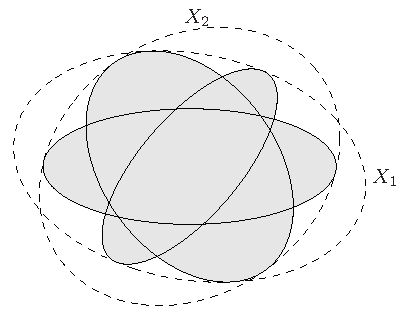
\includegraphics[width=.55\textwidth]{figures/ch04-10.pdf}
\caption*{图4.10\quad 问题（4.63）的几何解释。三个阴影椭球对应数据 $A_1,A_2,A_3\in\mathbf S_{++}^2$；Pareto最优点对应包含它们的极小椭球。边界标为 $X_1,X_2$ 的两个椭球，是用不同权重矩阵 $W_1,W_2$ 求解SDP（4.64）所得的两个极小椭球。}
\end{figure}
于是 $A\preceq B$ 当且仅当 $\mathcal E_A\subseteq\mathcal E_B$。问题（4.63）的Pareto最优点 $X$，对应一个包含与 $A_1,\ldots,A_m$ 关联椭球的极小椭球。图4.10给出一例。
\end{origexample}

\subsection{多准则优化}
向量优化问题的锥为 $K=\R_+^q$ 时，称为多准则或多目标优化问题。$f_0$ 的分量记为 $F_1,\ldots,F_q$，可解释为 $q$ 个不同的标量目标，我们希望每一个都尽可能小。称 $F_i$ 为问题的第 $i$ 个目标。多准则问题凸，要求 $f_1,\ldots,f_m$ 凸、$h_1,\ldots,h_p$ 仿射，并且目标 $F_1,\ldots,F_q$ 均凸。

多准则问题是向量优化问题，所以§4.7.1至§4.7.4的全部内容都适用。不过，多准则问题的解释可以更具体。对可行点 $x$，可将 $F_i(x)$ 看作按第 $i$ 个目标评定的得分或价值。若 $x,y$ 均可行，$F_i(x)\le F_i(y)$ 表示按第 $i$ 个目标 $x$ 至少与 $y$ 一样好；$F_i(x)<F_i(y)$ 表示按第 $i$ 个目标 $x$ 优于或胜过 $y$。若 $x,y$ 均可行，且 $F_i(x)\le F_i(y)$（$i=1,\ldots,q$），并至少存在一个 $j$ 使 $F_j(x)<F_j(y)$，就称 $x$ 优于或支配 $y$。粗略地说，$x$ 在所有目标上都不逊于 $y$，并至少在一个目标上胜过 $y$，就称 $x$ 更好。

多准则问题的最优点 $x^\star$ 满足，对每个可行 $y$，
\[
F_i(x^\star)\le F_i(y),\quad i=1,\ldots,q.
\]

% Source PDF page 196 (printed p. 182)
换言之，对 $j=1,\ldots,q$，$x^\star$ 同时是各个标量问题
\[
\begin{array}{ll}\text{最小化}&F_j(x)\\\text{约束为}&f_i(x)\le0,\quad i=1,\ldots,m,\\&h_i(x)=0,\quad i=1,\ldots,p\end{array}
\]
的最优点。存在最优点时，称各目标不竞争，因为无需在目标之间妥协：每个目标都达到即使忽略其他目标也只能达到的最小值。

Pareto最优点 $x^{\mathrm{po}}$ 满足：若 $y$ 可行，且 $F_i(y)\le F_i(x^{\mathrm{po}})$（$i=1,\ldots,q$），则 $F_i(x^{\mathrm{po}})=F_i(y)$（$i=1,\ldots,q$）。也就是说，一个点Pareto最优，当且仅当它可行且不存在更好的可行点。特别地，若可行点不Pareto最优，则至少存在另一个更好的可行点。因此寻找好的点时，显然只需搜索Pareto最优点。

\subsubsection*{权衡分析}
设 $x,y$ 为Pareto最优点，例如
\[
\begin{aligned}
F_i(x)&<F_i(y),&&i\in\mathcal A,\\
F_i(x)&=F_i(y),&&i\in\mathcal B,\\
F_i(x)&>F_i(y),&&i\in\mathcal C,
\end{aligned}
\]
其中 $\mathcal A\cup\mathcal B\cup\mathcal C=\{1,\ldots,q\}$。换言之，$\mathcal A$ 是 $x$ 胜过 $y$ 的目标指标集，$\mathcal B$ 是两点打平的目标集，$\mathcal C$ 是 $y$ 胜过 $x$ 的目标集。若 $\mathcal A,\mathcal C$ 均为空，两点的全部目标值相同；否则两者都必须非空。因此，比较两个Pareto最优点时，要么两者性能相同，即全部目标相等；要么各自至少在一个目标上胜过对方。

比较 $x$ 与 $y$ 时，可以说我们用 $i\in\mathcal C$ 的较差目标值，换取了 $i\in\mathcal A$ 的较好目标值。最优权衡分析，或简称权衡分析，研究为了改善某些目标，必须让另一个或多个目标变差多少；更一般地，它研究哪些目标值组合可达。

例如，考虑双准则问题。设 $x$ 为Pareto最优点，目标值为 $F_1(x),F_2(x)$。我们可以问：为了找到满足 $F_1(z)\le F_1(x)-a$ 的可行点 $z$，$F_2(z)$ 必须增大多少，其中 $a>0$ 为常数。粗略地说，这是问为了让第一个目标改善 $a$，必须在第二个目标上支付多少代价。若 $F_1$ 的小幅下降需要接受 $F_2$ 的大幅上升，就说在Pareto最优值 $(F_1(x),F_2(x))$ 附近，两目标之间的权衡很强。反之，若 $F_2$ 只需小幅上升即可让 $F_1$ 大幅下降，就说附近的权衡很弱。

也可以考虑以第一个目标的较差性能，换取第二个目标的改善。这时要在 $F_1(z)\le F_1(x)+a$ 的条件下，考察 $F_2(z)$ 可以降低多少，其中 $a>0$。

% Source PDF page 197 (printed p. 183)
此时获得的第二目标收益，就是 $F_2$ 相对于 $F_2(x)$ 的下降。若收益很大，即 $F_1$ 小幅增加换得 $F_2$ 大幅下降，就说目标之间权衡很强；若收益很小，就说在Pareto最优值 $(F_1(x),F_2(x))$ 附近权衡很弱。

\subsubsection*{最优权衡曲面}
多准则问题的Pareto最优值集，通常在 $q>2$ 时称为最优权衡曲面，在 $q=2$ 时称为最优权衡曲线。（接受一个非Pareto最优点是不明智的，因此权衡分析可以限于Pareto最优点。）权衡分析有时也称为探索最优权衡曲面。（最优权衡曲面通常、但并非总是通常意义下的曲面。例如，问题有最优点时，最优权衡曲面只包含最优值这一个点。）

最优权衡曲线很容易解释。第185页图4.11给出凸双准则问题的一例。由曲线可以直观理解两目标的权衡。
\begin{itemize}
\item 右端点给出完全不考虑 $F_1$ 时，$F_2$ 的最小可能值。
\item 左端点给出完全不考虑 $F_2$ 时，$F_1$ 的最小可能值。
\item 找曲线与竖线 $F_1=\alpha$ 的交点，可知为达到 $F_1\le\alpha$，$F_2$ 必须多大。
\item 找曲线与横线 $F_2=\beta$ 的交点，可知为达到 $F_2\le\beta$，$F_1$ 必须多大。
\item 曲线上某点，即某个Pareto最优值处的斜率，反映两目标的局部最优权衡。斜率陡峭处，$F_1$ 的小变化伴随 $F_2$ 的大变化。
\item 曲率大的点，是一个目标的小幅下降只能通过另一个目标的大幅增加实现的位置。这就是常说的权衡曲线“膝点”，在许多应用中代表良好的折中解。
\end{itemize}
这些解释都容易推广到权衡曲面，不过超过三个目标的曲面难以可视化。

\subsubsection*{多准则问题的标量化}
通过加权和目标
\[
\lambda^\T f_0(x)=\sum_{i=1}^q\lambda_iF_i(x),\qquad\lambda\succ0
\]
对多准则问题进行标量化时，可以将 $\lambda_i$ 解释为赋予第 $i$ 个目标的权重。

% Source PDF page 198 (printed p. 184)
权重 $\lambda_i$ 可看作衡量希望 $F_i$ 较小的程度，或反对 $F_i$ 较大的程度。特别地，若希望 $F_i$ 小，应取较大的 $\lambda_i$；若对 $F_i$ 的关心小得多，可取较小的 $\lambda_i$。比值 $\lambda_i/\lambda_j$ 可解释为第 $i$ 个目标相对于第 $j$ 个的权重或重要性。也可将它看作两目标的兑换率，因为在加权目标中，$F_i$ 下降 $\alpha$，等同于 $F_j$ 上升 $(\lambda_i/\lambda_j)\alpha$。

这些解释为探索最优权衡曲面时设置和调整权重提供直觉。例如，权重向量 $\lambda\succ0$ 得到Pareto最优点 $x^{\mathrm{po}}$，目标值为 $F_1(x^{\mathrm{po}}),\ldots,F_q(x^{\mathrm{po}})$。为寻找可能的新Pareto最优点，让第 $k$ 个目标改善，而其他目标可能变差，构造新权重向量 $\widetilde\lambda$，满足
\[
\widetilde\lambda_k>\lambda_k,\qquad\widetilde\lambda_j=\lambda_j,\quad j\ne k,\quad j=1,\ldots,q,
\]
即增大第 $k$ 个目标的权重。得到的新Pareto最优点 $\widetilde x^{\mathrm{po}}$ 满足 $F_k(\widetilde x^{\mathrm{po}})\le F_k(x^{\mathrm{po}})$，通常为严格小于，即第 $k$ 个目标改善。

还可看到，在最优权衡曲面光滑的任意一点，$\lambda$ 是相应Pareto最优点处指向曲面内部的法向量。特别地，选择权重向量 $\lambda$ 并标量化，得到的Pareto最优点处，$\lambda$ 给出了目标间的局部权衡。

实际中，常依据上述直觉，逐次试调权重来探索最优权衡曲面。第5章将看到，标量化的基本思想，即最小化目标的加权和，再调整权重得到合适解，正是对偶性的核心。

\subsection{例子}
\subsubsection*{正则化最小二乘}
给定 $A\in\R^{m\times n}$、$b\in\R^m$，希望选择 $x\in\R^n$，同时考虑两个二次目标：
\begin{itemize}
\item $F_1(x)=\norm{Ax-b}_2^2=x^\T A^\T Ax-2b^\T Ax+b^\T b$，衡量 $Ax$ 与 $b$ 的不匹配程度；
\item $F_2(x)=\norm{x}_2^2=x^\T x$，衡量 $x$ 的大小。
\end{itemize}
目标是寻找拟合较好，即 $F_1$ 小，同时幅度不大，即 $F_2$ 小的 $x$。可将其写成关于锥 $\R_+^2$ 的向量优化问题，即无约束双准则问题：
\[
\text{最小化（关于 }\R_+^2\text{）}\quad f_0(x)=(F_1(x),F_2(x)).
\]

% Source PDF page 199 (printed p. 185)
\begin{figure}[htbp]
\centering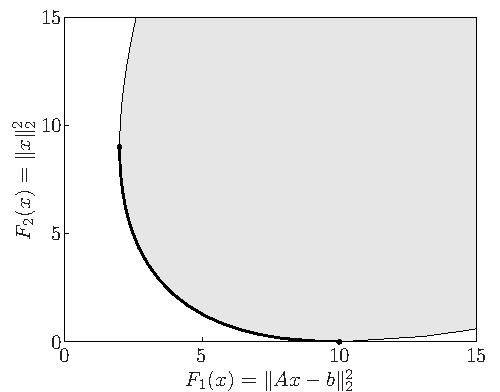
\includegraphics[width=.65\textwidth]{figures/ch04-11.pdf}
\caption*{图4.11\quad 正则化最小二乘问题的最优权衡曲线。阴影区域为可达值 $(\norm{Ax-b}_2^2,\norm{x}_2^2)$ 的集合。加粗的最优权衡曲线是边界的左下部分。}
\end{figure}
取 $\lambda_1>0$、$\lambda_2>0$，最小化标量加权目标，就可将问题标量化：
\[
\begin{aligned}
\lambda^\T f_0(x)&=\lambda_1F_1(x)+\lambda_2F_2(x)\\
&=x^\T(\lambda_1A^\T A+\lambda_2I)x-2\lambda_1b^\T Ax+\lambda_1b^\T b,
\end{aligned}
\]
从而得到
\[
x(\mu)=(\lambda_1A^\T A+\lambda_2I)^{-1}\lambda_1A^\T b
=(A^\T A+\mu I)^{-1}A^\T b,
\]
其中 $\mu=\lambda_2/\lambda_1$。对任意 $\mu>0$，此点都对双准则问题Pareto最优。$\mu$ 可解释为赋予 $F_2$ 相对于 $F_1$ 的权重。

这种方法能得到全部Pareto最优点，唯独缺少对应极端情形 $\mu\to\infty$ 与 $\mu\to0$ 的两个点。第一种情形的Pareto最优解为 $x=0$，可用 $\lambda=(0,1)$ 标量化得到。另一端的Pareto最优解为 $A^\dagger b$，其中 $A^\dagger$ 为 $A$ 的伪逆。它可作为 $\mu\to0$，即 $\lambda\to(1,0)$ 时标量化问题最优解的极限得到。（§6.3.2还会讨论正则化最小二乘。）

图4.11展示问题数据为 $A\in\R^{100\times10}$、$b\in\R^{100}$ 的正则化最小二乘问题的最优权衡曲线及可达值集，另见习题4.50。

\subsubsection*{投资组合优化中的风险收益权衡}
第155页的经典Markowitz投资组合问题自然可表述为双准则问题，目标为负的平均收益（因为希望最大化平均收益）和收益方差：

% Source PDF page 200 (printed p. 186)
\[
\begin{array}{ll}\text{最小化（关于 }\R_+^2\text{）}&(F_1(x),F_2(x))=(-\bar p^\T x,x^\T\Sigma x)\\\text{约束为}&\one^\T x=1,\quad x\succeq0.\end{array}
\]
构造对应的标量化问题时，不失一般性可取 $\lambda_1=1$、$\lambda_2=\mu>0$：
\[
\begin{array}{ll}\text{最小化}&-\bar p^\T x+\mu x^\T\Sigma x\\\text{约束为}&\one^\T x=1,\quad x\succeq0,\end{array}
\]
这是QP。同样可以得到全部Pareto最优投资组合，除去 $\mu\to0$ 与 $\mu\to\infty$ 对应的两个极限情形。粗略地说，前者不考虑收益方差，只求最大平均收益；后者不考虑平均收益，只求最小方差。若 $\bar p_k>\bar p_i$（$i\ne k$），即资产 $k$ 是唯一具有最大平均收益的资产，则 $\mu\to0$ 只对应组合 $x=e_k$，即全部投资集中在平均收益最高的资产。许多投资组合问题中，资产 $n$ 是无风险投资，确定收益为 $r_{\mathrm{rf}}$。若删去 $\Sigma$ 最后一行和最后一列（它们为零）后所得矩阵满秩，则另一端的Pareto最优组合为 $x=e_n$，即全部集中在无风险资产。

作为具体例子，考虑有4种资产的简单投资组合优化，其价格变化均值和标准差为
\begin{center}
\begin{tabular}{ccc}
\toprule 资产&$\bar p_i$&$\Sigma_{ii}^{1/2}$\\\midrule
1&$12\%$&$20\%$\\2&$10\%$&$10\%$\\3&$7\%$&$5\%$\\4&$3\%$&$0\%$\\\bottomrule
\end{tabular}
\end{center}
资产4无风险，确定收益为 $3\%$。资产3、2、1的平均收益依次增加，从 $7\%$ 到 $12\%$；标准差也依次增大，从 $5\%$ 到 $20\%$。资产之间相关系数为 $\rho_{12}=30\%$、$\rho_{13}=-40\%$、$\rho_{23}=0\%$。

图4.12给出此问题的最优权衡曲线，采用通常的画法，横轴为标准差，即方差平方根，纵轴为期望收益。下图展示每个Pareto最优点对应的最优资产配置向量 $x$。

这个简单例子的结果符合直觉。风险较小时，最优配置大部分是无风险资产，并混合少量其他资产。注意，负相关的资产3和资产1混合，提供了一定对冲，即在给定平均收益下减小方差。在权衡曲线另一端，追求较大平均收益的激进增长组合，将配置集中在平均收益和方差最大的资产1、2上。

% Source PDF page 201 (printed p. 187)
\begin{figure}[htbp]
\centering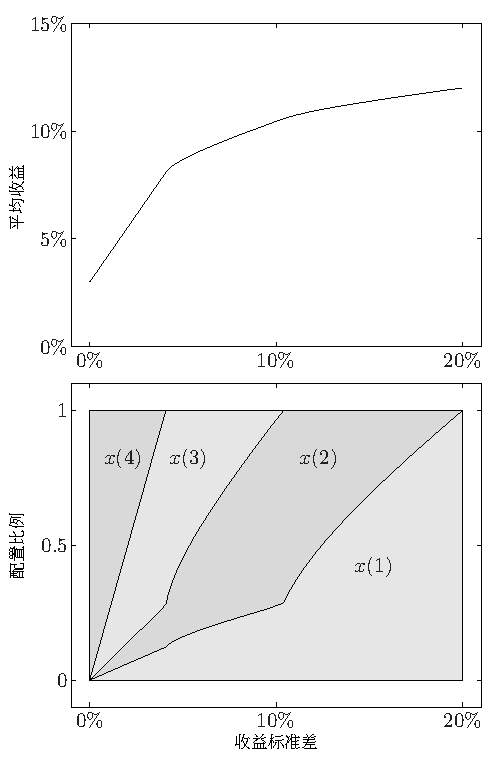
\includegraphics[width=.65\textwidth]{figures/ch04-12.pdf}
\caption*{图4.12\quad 上图：简单投资组合优化的最优风险收益权衡曲线。左端点对应全部投资于无风险资产，因而标准差为零。右端点对应全部投资于平均收益最高的资产1。下图：对应的最优配置。}
\end{figure}

% Source PDF page 202 (printed p. 188)
\section*{文献说明}
\addcontentsline{toc}{section}{文献说明}
线性规划自20世纪40年代以来得到广泛研究，是许多优秀著作的主题，包括Dantzig [Dan63]、Luenberger [Lue84]、Schrijver [Sch86]、Papadimitriou和Steiglitz [PS98]、Bertsimas和Tsitsiklis [BT97]、Vanderbei [Van96]，以及Roos、Terlaky和Vial [RTV97]。Dantzig和Schrijver还详细介绍了线性规划史。较新的综述见Todd [Tod02]。

Schaible [Sch82, Sch83] 概述了分式规划，包括线性分式问题及凸凹分式问题等推广，见习题4.7。例4.7的经济增长模型出自von Neumann [vN46]。

二次规划研究始于20世纪50年代，例如Frank和Wolfe [FW56]、Markowitz [Mar56]、Hildreth [Hil57]；部分动机来自第155页的投资组合优化问题（Markowitz [Mar52]），以及第154页的随机成本LP，见Freund [Fre56]。

二阶锥规划较晚才引起关注，始于Nesterov和Nemirovski [NN94, §6.2.3]。关于SOCP理论和应用的综述，见Alizadeh和Goldfarb [AG03]、Ben-Tal和Nemirovski [BTN01, lecture 3]（其中称为锥二次规划），以及Lobo、Vandenberghe、Boyd和Lebret [LVBL98]。

鲁棒线性规划以及更一般的鲁棒凸优化，始于Ben-Tal和Nemirovski [BTN98, BTN99] 与El Ghaoui和Lebret [EL97]。Goldfarb和Iyengar [GI03a, GI03b] 讨论鲁棒QCQP及其在投资组合优化中的应用。El Ghaoui、Oustry和Lebret [EOL98] 专门研究鲁棒半正定规划。

几何规划自20世纪60年代起为人所知。Duffin、Peterson和Zener [DPZ67] 与Zener [Zen71] 最先倡导将其用于工程设计。Peterson [Pet76] 与Ecker [Eck80] 介绍了20世纪70年代的进展。这些文章和书籍还包括工程应用例子，特别是化学工程和土木工程。Fishburn和Dunlop [FD85]、Sapatnekar、Rao、Vaidya和Kang [SRVK93]，以及Hershenson、Boyd和Lee [HBL01] 将几何规划用于集成电路设计。第163页的悬臂梁设计例子取自Vanderplaats [Van84, page 147]。第165页Perron--Frobenius特征值的变分刻画证明见Berman和Plemmons [BP94, page 31]。

Nesterov和Nemirovski [NN94, chapter 4] 将锥形式问题（4.49）作为非线性凸优化的一种标准问题格式引入。Ben-Tal和Nemirovski [BTN01] 进一步发展了锥规划方法，并介绍大量应用。

Alizadeh [Ali91] 与Nesterov和Nemirovski [NN94, §6.4] 最先系统研究半正定规划，并指出其在凸优化中的广泛应用。20世纪90年代，半正定规划的后续研究由组合优化、控制、通信与信号处理及其他工程领域的应用推动。组合优化见Goemans和Williamson [GW95]；控制见Boyd、El Ghaoui、Feron和Balakrishnan [BEFB94]、Scherer、Gahinet和Chilali [SGC97]、Dullerud和Paganini [DP00]；通信与信号处理见Luo [Luo03]、Davidson、Luo、Wong和Ma [DLW00, MDW$^+$02]。Wolkowicz、Saigal和Vandenberghe编辑的书 [WSV00]，以及Todd [Tod01]、Lewis和Overton [LO96]、Vandenberghe和Boyd [VB95] 的文章，提供了综述和广泛的参考文献。第170页给出简单例子的SDP与矩问题之间的联系，由Bertsimas和Sethuraman [BS00]、Nesterov [Nes00] 和Lasserre [Las02] 详细研究。最快混合马尔可夫链问题出自Boyd、Diaconis和Xiao [BDX04]。

多准则优化和Pareto最优性是经济学的基本工具，见Pareto [Par71]、Debreu [Deb59]、Luenberger [Lue95]。例4.9的结果称为Gauss--Markov定理，见Kailath、Sayed和Hassibi [KSH00, page 97]。
